\section{Governance-constrained H/A/C benchmark}
\label{sec:benchmark}

Let tasks $i\in I$ have duration $d_i$, priority $p_i$, value $v_i$, region $r(i)$ and an allowed mode domain $D_i\subseteq\{\Hmode,\Amode,\Cmode\}$. Human-mandatory tasks exclude $\Amode$. The assignment and explicit mode-violation count are
\begin{equation}
 y_i\in D_i,\qquad H(y)=\sum_{i\in I}\ind[y_i\notin D_i].
 \label{eq:mode}
\end{equation}
Costs are $C(y)=\sum_i d_i c_{i,y_i}$. Review-required AI-only tasks contribute one unit and collaborative tasks one quarter,
$R(y)=\sum_i r_i(\ind[y_i=\Amode]+.25\ind[y_i=\Cmode])$, with overflow $R_+(y)=[R(y)-B_R]_+$.

Tasks form workflow clusters $k$. Writing $n_k^C$ for the collaboration count, $h_k$ for its threshold and $m_k$ for the number of distinct modes, the cluster term is
\begin{equation}
 G(y)=\sum_k\!\left(B_k\ind[n_k^C\ge h_k]-A_k\ind[\forall i\!\in\!k:y_i=\Amode]-J_k(m_k-1)_+\right).
 \label{eq:cluster}
\end{equation}
This distinguishes workflow complementarity from an assumption that every individual collaborative assignment is beneficial. A coded exposure term $P_{\rm exp}(y)=2\operatorname{sd}_{r}(a_r)$ penalizes dispersion in regional AI-only rates $a_r$. It is a transparent benchmark regularizer, not a normative fairness definition.

For each correlated scenario $\omega\in\Omega$, the evaluator constructs mode-dependent regional human and AI loads, success $s_{i\omega}(y_i)$, and positive capacity overflow $O_\omega(y)$. Collaboration draws $.45$ human and $.65$ AI load; its success blends regional human/AI factors $.55/.45$ and an AI shock. Define empirical service and capacity failure rates
\begin{equation}
 q_s(y)=\frac1{|\Omega|}\sum_\omega \ind\!\left[\frac{\sum_i p_i s_{i\omega}(y_i)}{\sum_i p_i}<.70\right],\quad
 q_c(y)=\frac1{|\Omega|}\sum_\omega\ind[O_\omega(y)>0].
 \label{eq:chance}
\end{equation}
They implement empirical chance constraints with tolerance $\epsilon=.20$ rather than per-task service guarantees. The exact composite score is
\begin{align}
 S(y)={}&\frac1{|\Omega|}\sum_\omega\left(\sum_i v_i s_{i\omega}(y_i)-C(y)-4O_\omega(y)\right)+G(y)-P_{\rm exp}(y) \nonumber\\[-1mm]
 &-9R_+(y)-600H(y)-150[q_s(y)-.20]_+-45[q_c(y)-.20]_+ .
 \label{eq:score}
\end{align}
Composite feasibility is the conjunction $F(y)=\ind[H=0,R_+=0,q_s\le.20,q_c\le.20]$. Keeping $H$ and $F$ separate is essential: the frozen incumbents have no disallowed modes, yet five exceed a stochastic or review tolerance.

\begin{table}[t]
\centering
\caption{Five factor families in the implemented evaluator.}
\label{tab:factorfamilies}
\scriptsize
\begin{tabularx}{\linewidth}{@{}p{0.20\linewidth}p{0.30\linewidth}X@{}}
\toprule
Family & Representative term & Operational interpretation \\
\midrule
Governance & $y_i\in\{H,A,C\}$; $H(y)=0$ & Human-mandatory tasks may not be AI-only. \\
Reliability & $q_s,q_c\le\epsilon$ & Scenario service and regional capacity remain within tolerances. \\
Oversight/exposure & $[R(y)-B_R]_+$; $2\,\mathrm{sd}(a_r)$ & Review capacity and regional AI-use dispersion are priced. \\
Complementarity & $B_k\mathbf1[n^C_k\ge h_k]-A_k\mathbf1[\mathbf y_k=A]-J_k(m_k-1)_+$ & Workflow-level collaboration rewards and handoff/all-AI penalties. \\
Evidence eligibility & gain, disagreement, strict core, $p_Q^\star/p_U^\star$ & Quantum evidence is interpreted only inside a classically characterized retained set. \\
\bottomrule
\end{tabularx}
\end{table}

\begin{figure}[t]
  \centering
  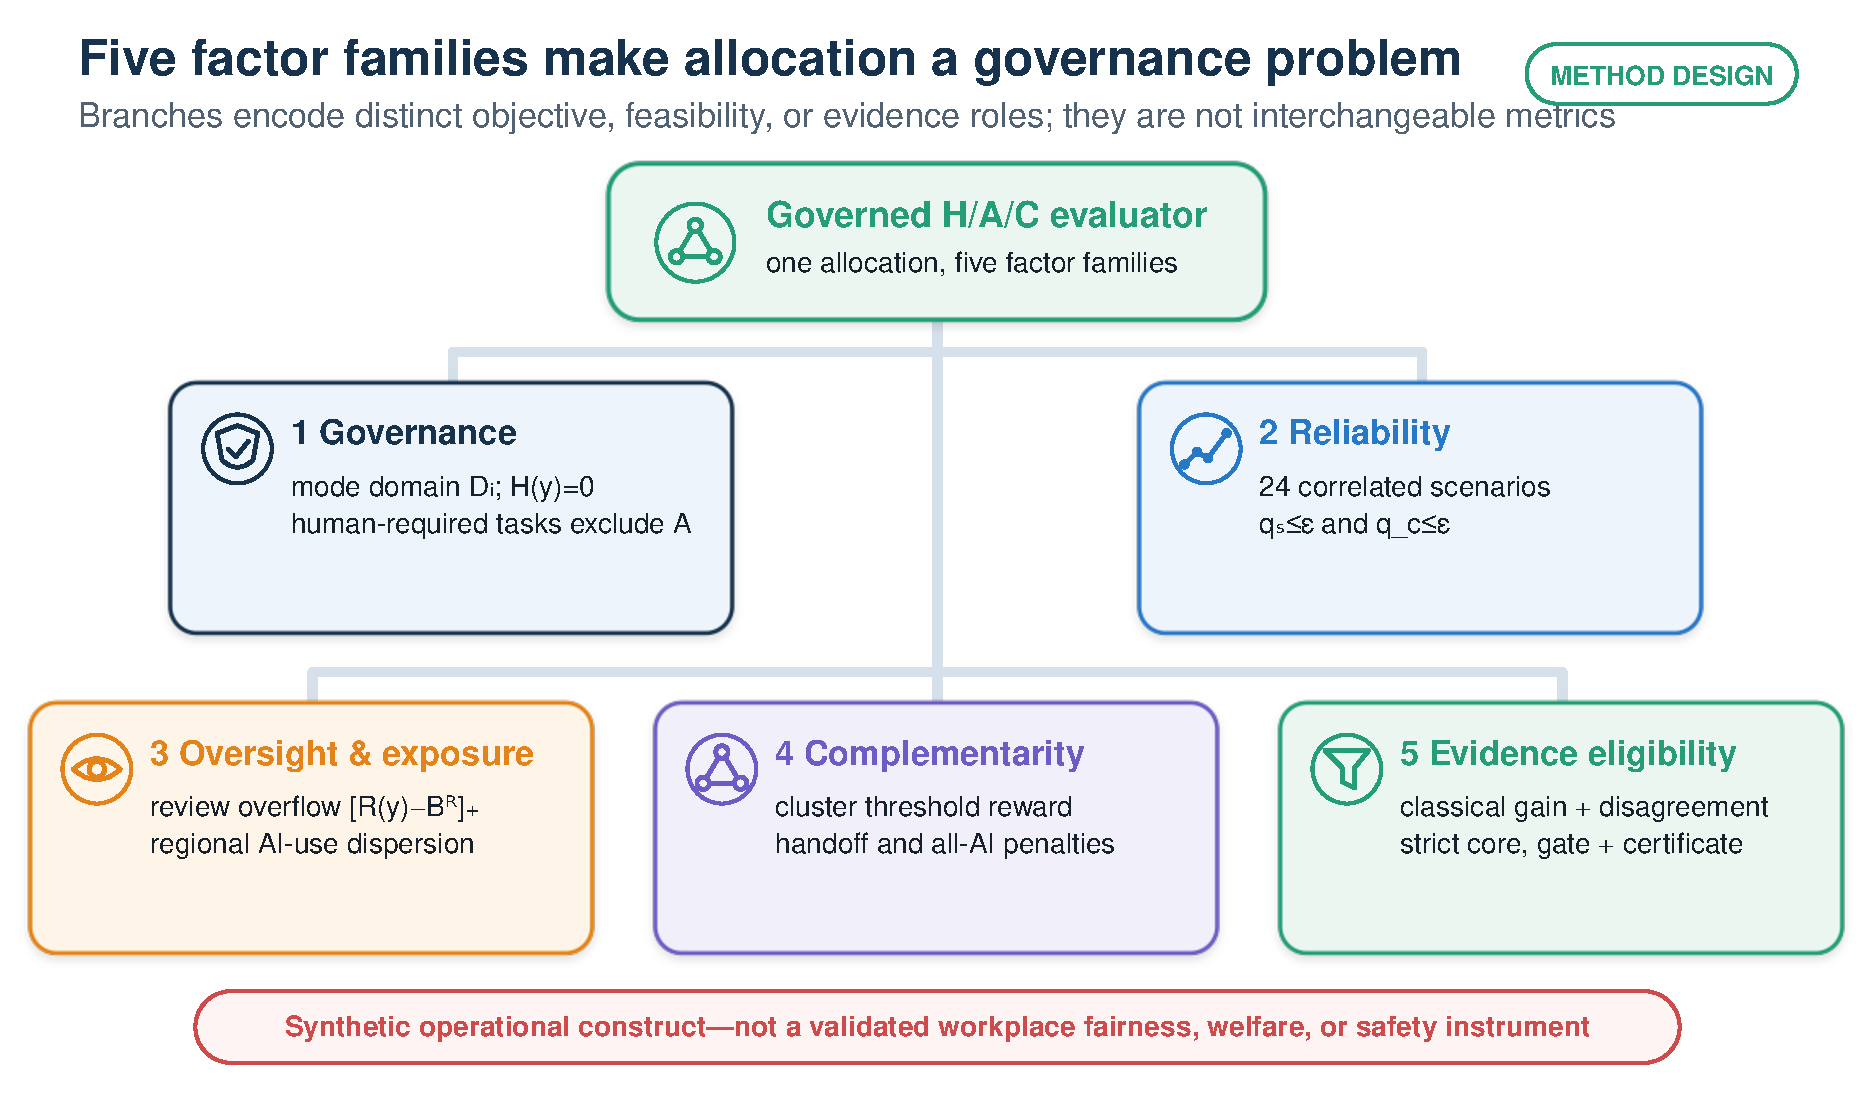
\includegraphics[width=\linewidth]{figs/fig2_benchmark_taxonomy.pdf}
  \caption{Five benchmark factor families. The exposure term is a coded dispersion regularizer, not a validated fairness construct; all variables and coefficients are specified in Appendix~\ref{app:benchmark}.}
  \label{fig:taxonomy}
\end{figure}


The five families in \cref{tab:factorfamilies,fig:taxonomy} are deliberately heterogeneous: governance, stochastic reliability, oversight/exposure, organizational complementarity, and evidence eligibility. Appendix~\ref{app:benchmark} gives every implemented formula, its plain-language meaning, status and literature connection. All numerical coefficients are frozen synthetic benchmark choices; none is presented as a learned social welfare weight or calibrated workplace threshold.
